%% Package and Class "uiucthesis2021" for use with LaTeX2e.
\documentclass[letterpage,11pt]{article}

\usepackage[acronym,toc]{glossaries}
\include{acros}

\usepackage{xspace}
\usepackage{graphicx}
\graphicspath{{images/}}
\usepackage[title,titletoc]{appendix}

\usepackage{placeins}
\usepackage{booktabs} % nice rules (thick lines) for tables
\usepackage{array}
\usepackage{microtype} % improves typography for PDF

\usepackage[hyphens]{url}
\usepackage[hidelinks]{hyperref}
\usepackage{caption}
\usepackage{subcaption}
\usepackage{hhline}
\usepackage{amsmath}
\usepackage{amssymb}
\usepackage{mathtools}
\allowdisplaybreaks
\usepackage{color}
\usepackage{multirow}
\usepackage{siunitx}
\usepackage{xfrac}
\usepackage{bm}

\usepackage{threeparttable, tablefootnote}

\usepackage{environ}
\makeatletter

\usepackage{tabularx}
\usepackage{float}
\usepackage{enumitem}
\usepackage{diagbox}
\usepackage{courier}
\usepackage{pdflscape}

\usepackage{cleveref}
\usepackage{datatool}
\usepackage[numbers]{natbib}
\usepackage{notoccite}
\usepackage{tikz}

\usepackage[ruled,linesnumbered,lined]{algorithm2e}
\SetArgSty{textrm}

\begin{document}

\title{Literature Review}
\author{Sun Myung Park}

\maketitle

{
  \hypersetup{linkcolor=black}
  \tableofcontents
}
\pagebreak

\section{Digital Twins}

\textit{Digital Twin Concepts with Uncertainty for Nuclear Power Applications}
\cite{kochunas_digital_2021}

Key characteristics of digital twins:
%
\begin{itemize}
  \item High-fidelity simulations
  \item Integration of calculated and measured quantities
  \item Detailed equivalence with a unique physical system
  \item Application over a product's life cycle
\end{itemize}

According to Kochunas \& Huan, three types of digital representations exist:
%
\begin{itemize}
  \item Digital model: May or may not be associated with a physical asset. Need not integrate with
    physically measured or sensed quantities. In contrast with the digital twin, information
    generated with the digital model is not automatically integrated with the physical asset.
  \item Digital shadow: Extends the digital model by incorporating information from an existing
    physical asset to update the digital model. Digital representations of historic facilities that
    no longer exist qualify as digital shadows.
  \item Digital twin: Closed loop of information exchange between physical asset and the digital
    representation. Exchanges information in real-time with the physical system to update its state
    and perform predictive calculations that are then used to inform decisions and control actions
    on the physical asset.
\end{itemize}

\begin{figure}[htb]
  \centering
  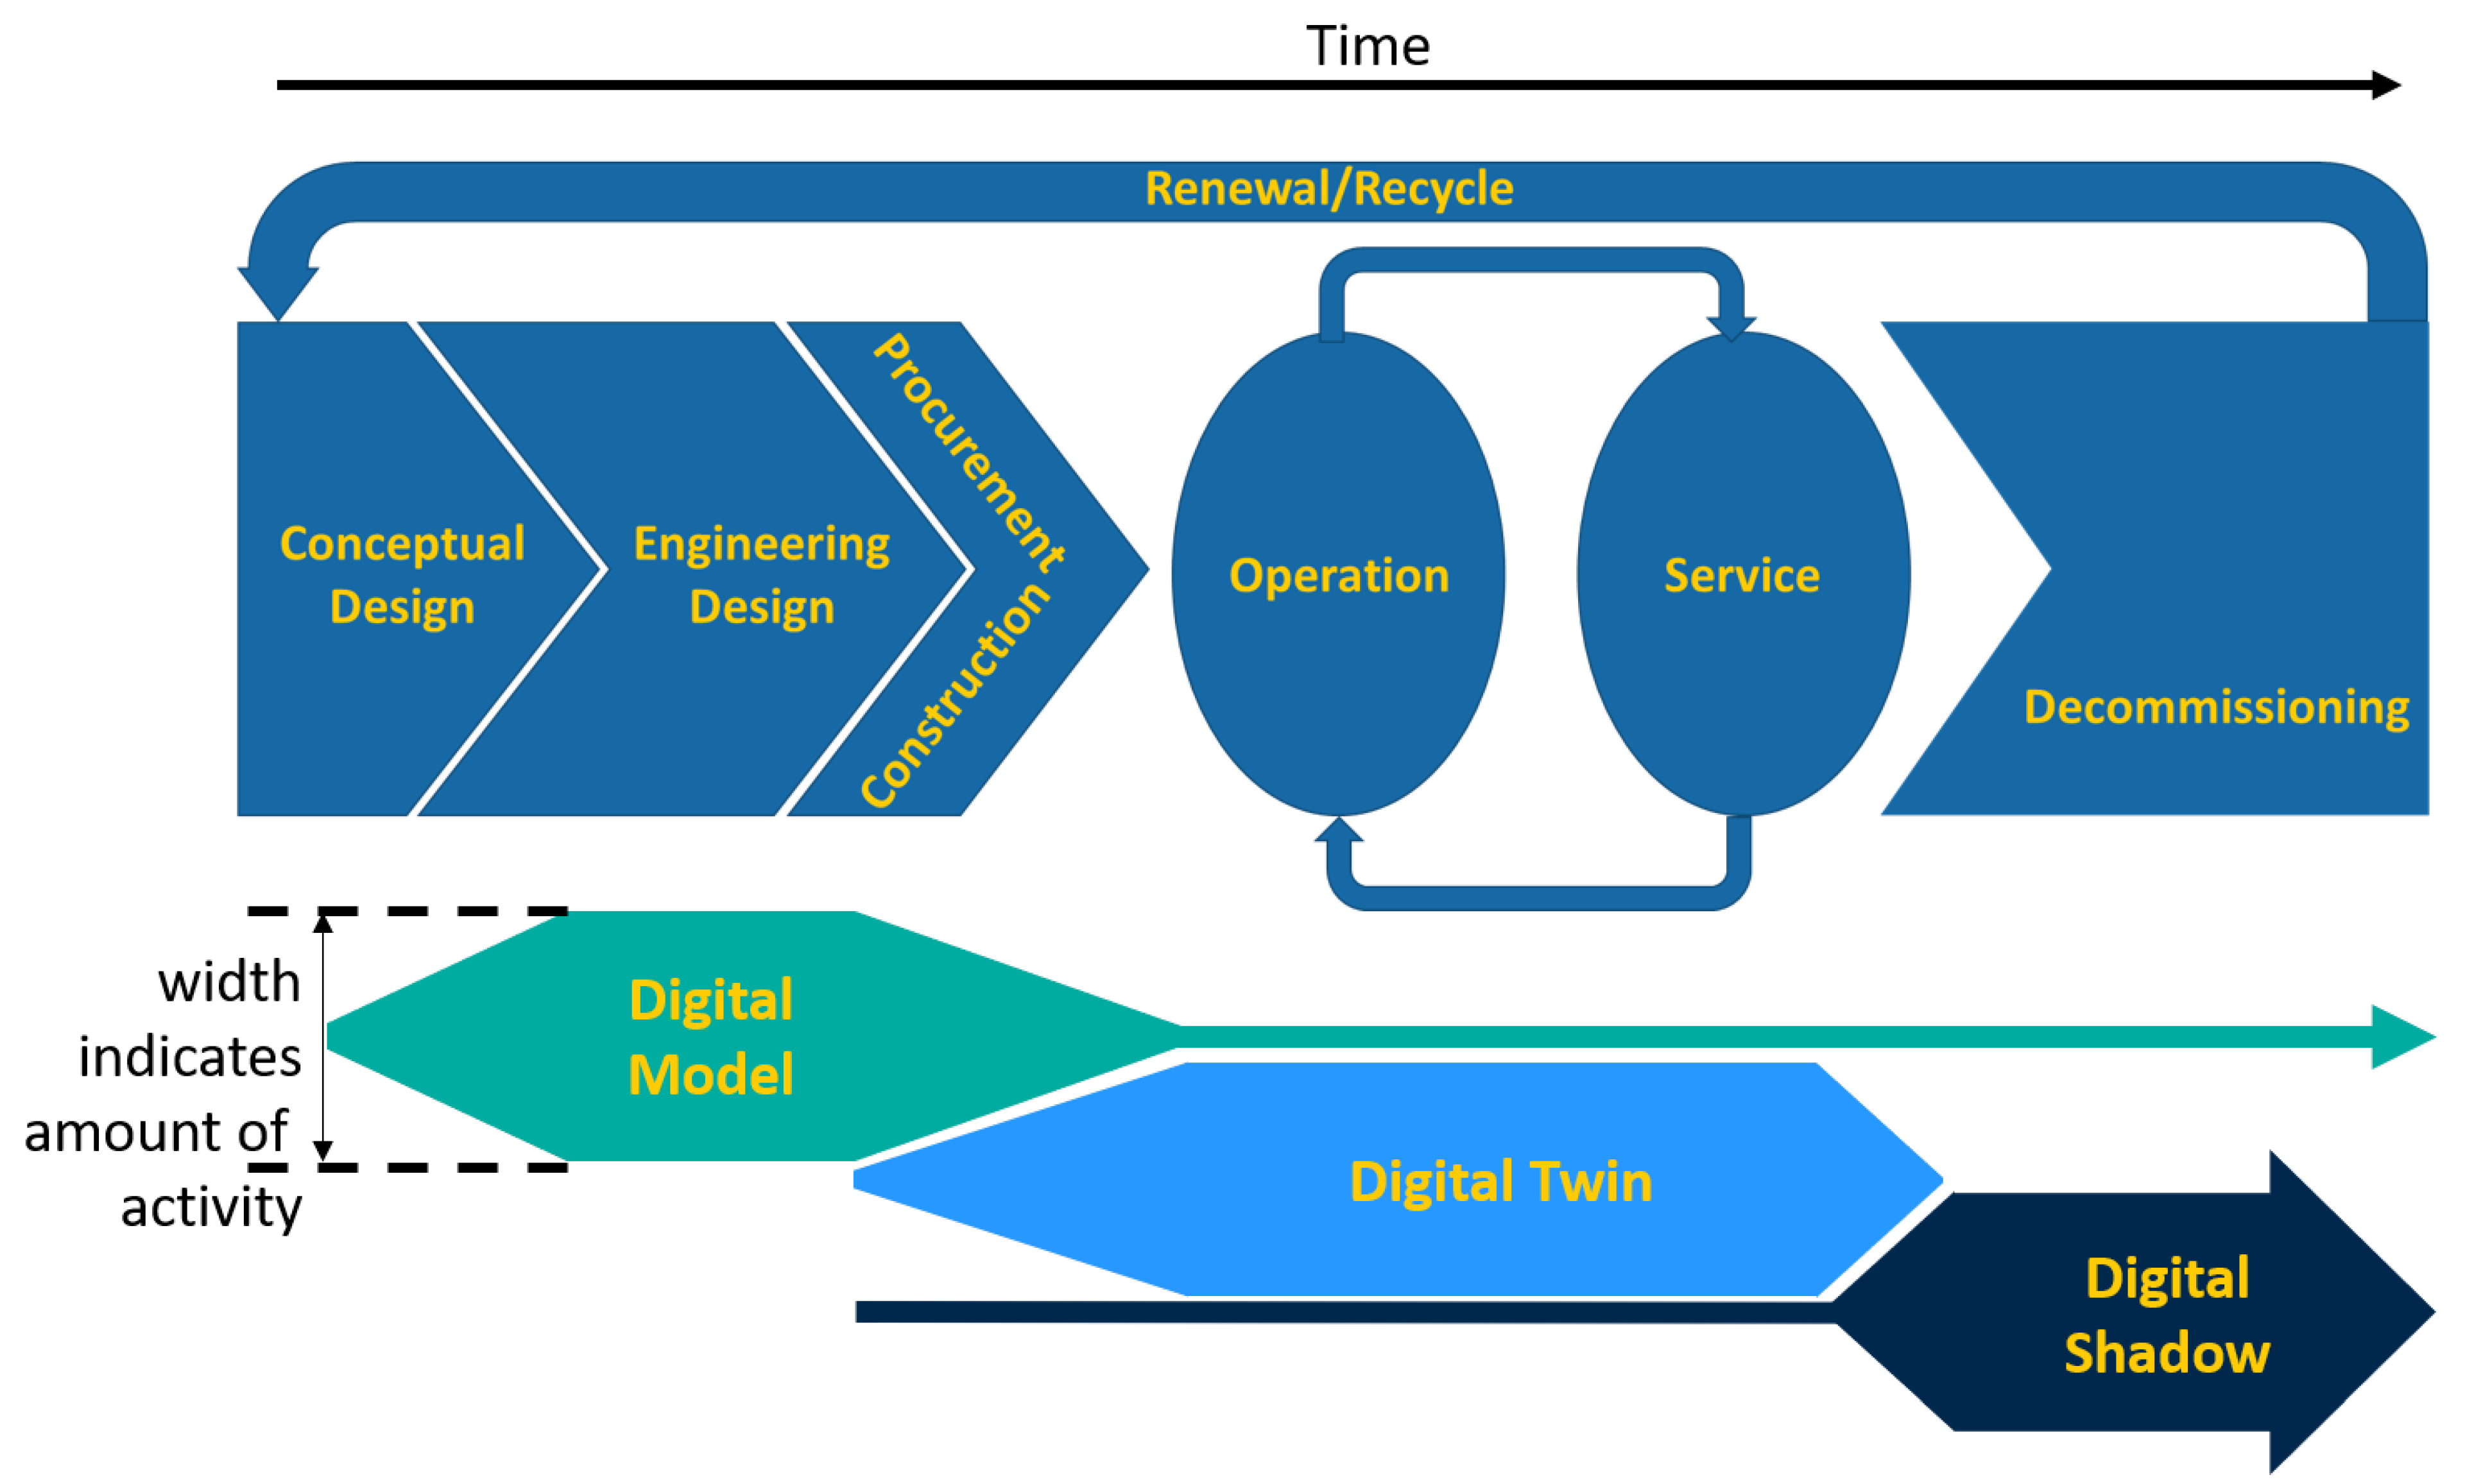
\includegraphics[width=\textwidth]{digital-twin-life-cycle}
  \caption{Illustration of physical asset life cycle phases and associated lifetimes and activity
  of the digital model, twin, and shadow.}
\end{figure}

Enabling technologies for digital twins of nuclear power systems:
%
\begin{itemize}
  \item Systems dynamics modeling: Can run in real-time, but needs novel methods for adapting
    models coefficients to better match a physical asset's behavior.
  \item Model-based controllers: May be developed to support autonomous control and operation.
    May be comprised of physics, statistical, data-driven, and ML models. Easier to justify for
    safey licensing than model-free controllers like PID.
  \item Automated ROM construction: Need automated ROM construction tools with ease of use and
    flexibility for use in digital twins.
  \item Functional mockup interface: Flexible software interface to facilitate model exchange and
    co-simulation.
\end{itemize}

High-fidelity models may be utilized as offline, on-demand capabilities to provide corrections to
low-fidelity digital twins.

Challenges for digital twins:
%
\begin{itemize}
  \item Information security
  \item Integration with prognostics and health management
  \item Data collection, curation, transmission, and integration
  \item Integration with risk assessments
\end{itemize}

\pagebreak
\bibliographystyle{ieeetr}
\bibliography{bibliography}

\end{document}
%%
